\section{Solution}
\label{sec:solution}
\subsection{Exercise 01}
We do not have any presentable results for exercise 1.
\subsection{Exercise 02}

\begin{itemize}
    \item[a)]
    We were supposed to implement both the euler scheme and the verlet scheme to calculate the trajectories of two masses.
    Those two masses acted a gravitational pull onto each other.
    The equation by which we were supposed to model the attraction is the Newton law of gravitation 
    \begin{equation}
        \vec{F}(\vec{r_1}, \vec{r_2}) = -G \frac{m_1 m_2}{|\vec{r_1} - \vec{r_2}} (\vec{r_1} - \vec{r_2})
    \end{equation}
    of which we set $G=1$ to make the equation dimensionless.\\\\
    As both schemes are recursive schemes our first thought was to implement the schemes recursively aswell.
    However, we quickly ran into problems as we tested out larger numbers of iterations for either big timescales $T$ or small stepsizes $h$.
    The recursive stack grew so large, that the program terminated with a segmentation error.\\
    We fixed this error by changing the recursive scheme to an iterative scheme in a somewhat ineffienct way.
    Another effiency problem that we encountered is that we open, write and close the .csv file, in which we write the trajectory data, everytime we walk through the loop.
    We chose this way of implementing the data saving process as we also ran into a segmentation error when we just dumped all our trajectory data in one big array.
    We would be happy to hear recommendations on how to improve the effiency of our code regarding the issues we mentioned.\\\\
    You can see the results of our program, plotted with a python script in the figures below.
    Our result show that the orbit that the masses take is unstable.
    For the time frame $T=(0-10)$ they orbit each other in a rather close distance.
    Afterwhich they accelerate into different directions and take independent paths.
    In figure \autoref{fig:h_001_10} one can see the intial orbit of both masses, as this plot only show the path up until $T=10$.
    \begin{figure}
        \centering
        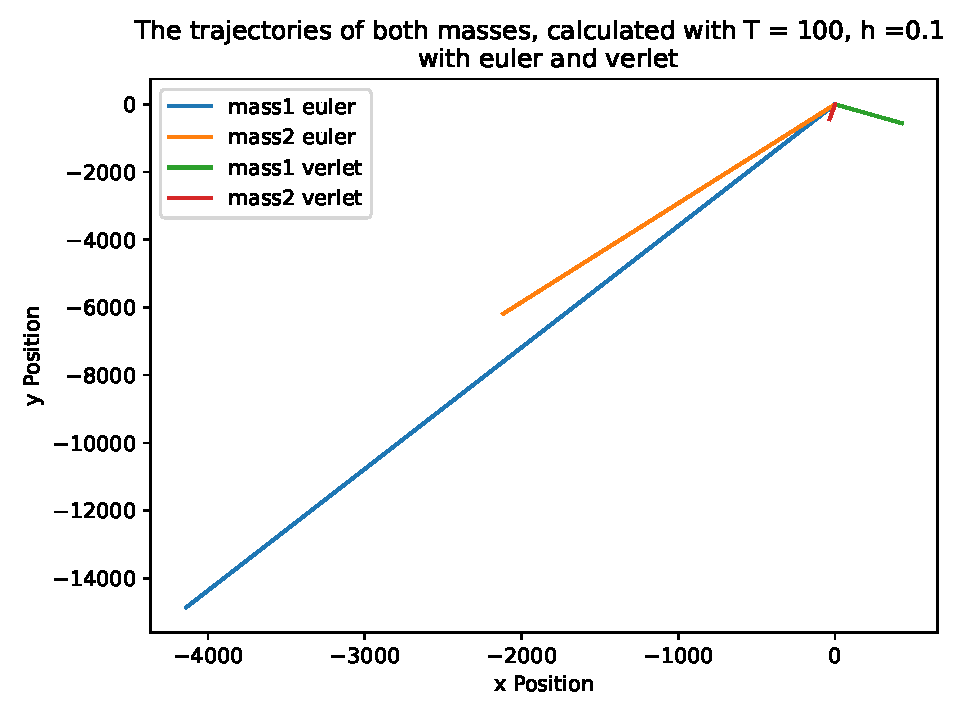
\includegraphics[width=\textwidth]{plots/plotsT_100_01/plota.pdf}
        \caption{The calculated trajectories with a stepsize of $h=0.1$ up to the time $T=100$.
        The trajectories of euler and verlet are displayed for bothe masses.}
        \label{fig:h_01_100}
    \end{figure}
    \begin{figure}
        \centering
        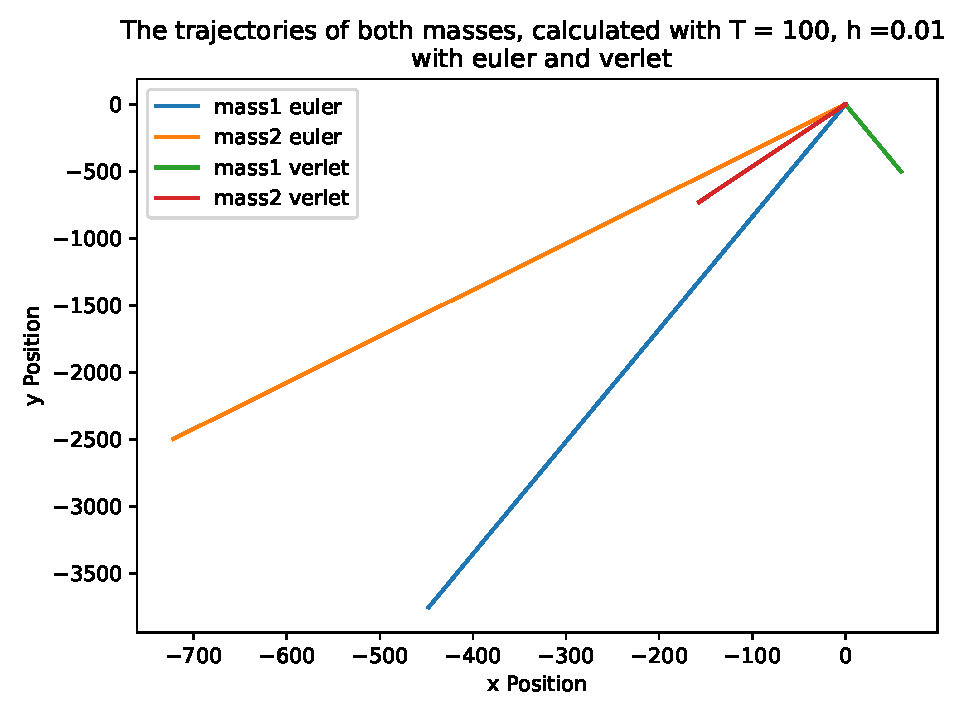
\includegraphics[width=\textwidth]{plots/plotsT_100_h_001/plota.pdf}
        \caption{The calculated trajectories with a stepsize of $h=0.01$ up to the time $T=100$.
        The trajectories of euler and verlet are displayed for bothe masses.}
        \label{}
    \end{figure}
    \begin{figure}
        \centering
        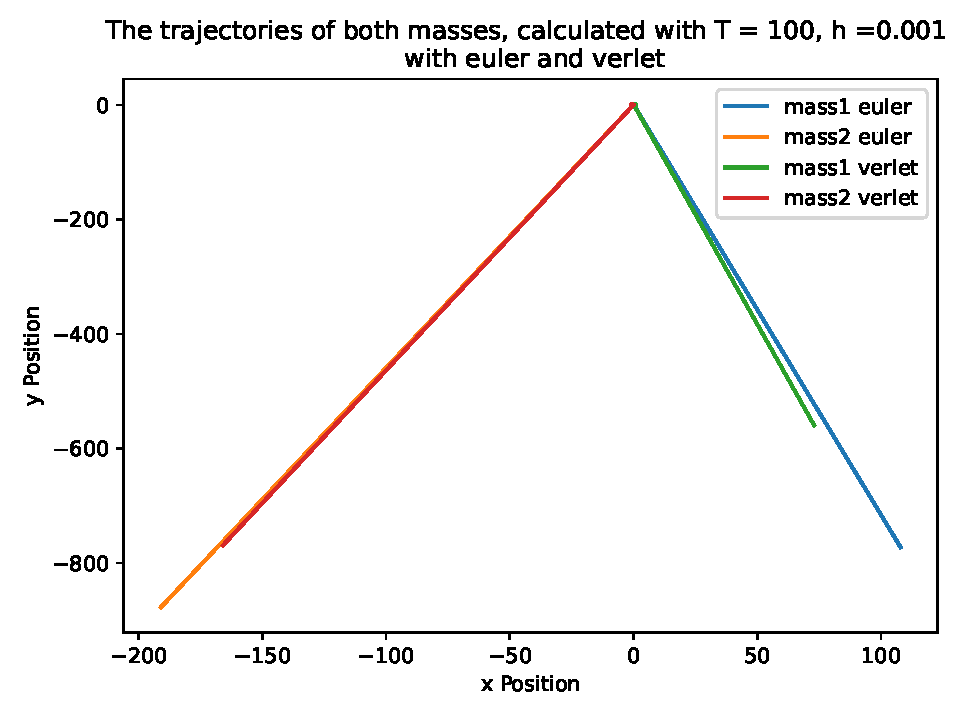
\includegraphics[width=\textwidth]{plots/plotsT_100_h_0001/plota.pdf}
        \caption{The calculated trajectories with a stepsize of $h=0.001$ up to the time $T=100$.
        The trajectories of euler and verlet are displayed for bothe masses.}
        \label{}
    \end{figure}
    \begin{figure}
        \centering
        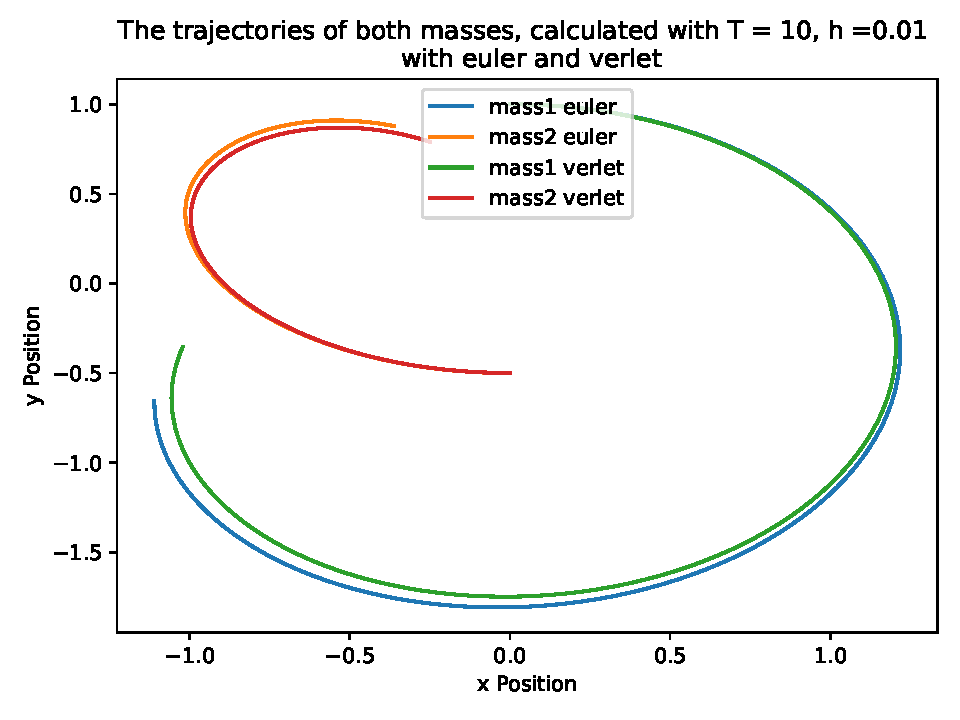
\includegraphics[width=\textwidth]{plots/plotsT_10_h_001/plota.pdf}
        \caption{The calculated trajectories with a stepsize of $h=0.01$ up to the time $T=10$.
        The trajectories of euler and verlet are displayed for bothe masses.}
        \label{fig:h_001_10}
    \end{figure}
\FloatBarrier

    \item[b)]
    The processing time of the schemes with different $T$ and $h$ values can be seen in the table \autoref{tab:timing}.
    For low numbers of iteration steps the time difference between euler and verlet is rather small.
    The euler scheme seems to be slower than the verlet scheme.
    The reason for this might be the inefficient way inwhich our program handles the saving process, or the schemes are not implemented in the most efficient maner.
    However, for larger numbers of computation, the verlet scheme is clearly slower than the euler scheme.
    \begin{table}
        \centering
        \caption{The time it took for the schemes to proces is listed in this table.
        }
        \begin{tabular}{ccc}
        \toprule
           Paramaters & euler$/s$ & verlet$/s$ \\
           \midrule
            $T=100$, $h=0.01$ & 71 & 69 \\ 
            $T=10$, $h=0.01$ & 5 & 4 \\
            $T=100$,$h=0.1$ & 6 & 5 \\
            $T=100$,$h=0.001$ & 418 & 468\\
           \bottomrule
        \end{tabular}
        \label{tab:timing}
    \end{table}
\FloatBarrier
    \item[c)]
    The back integration process did not seem to work in any of the given schemes.
    Both scheme generated trajectories that did not fit the intial path in any way.
    The trajectories with the same Paramaters as used in part a) of the exercise are shown in the figures below.
    \begin{figure}
        \centering
        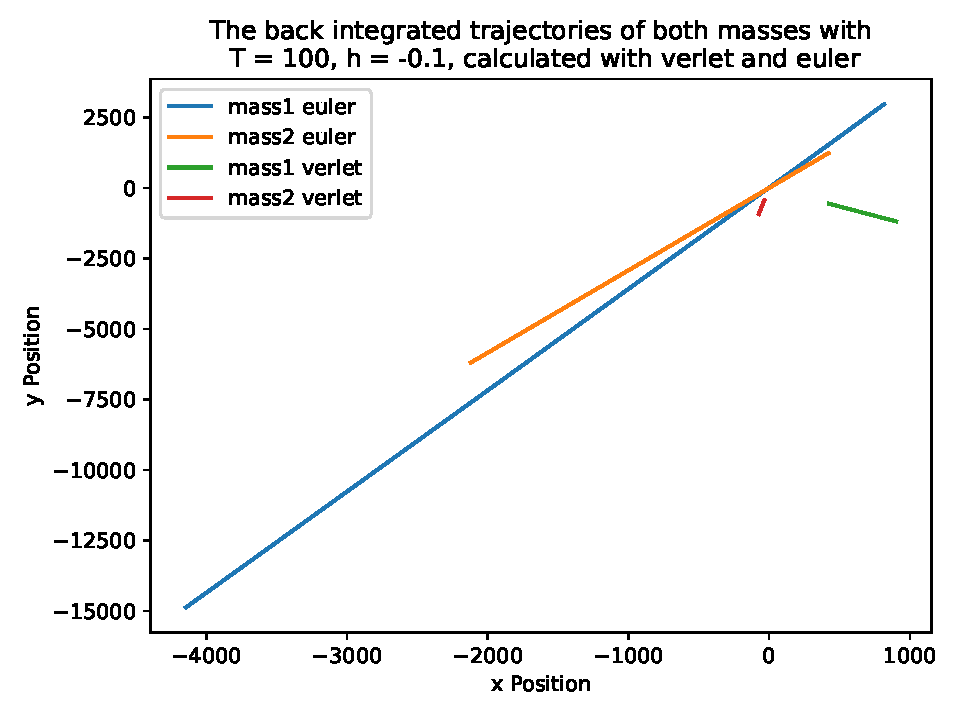
\includegraphics[width=\textwidth]{plots/plotsT_100_01/plotd.pdf}
        \caption{The calculated trajectories with a stepsize of $h=-0.1$ up to the time $T=100$.
        The trajectories of euler and verlet are displayed for bothe masses.
        This figures show just the back integrated trajectories from $T=(-100 - 0)$.}
        \label{fig:h_01_100}
    \end{figure}
    \begin{figure}
        \centering
        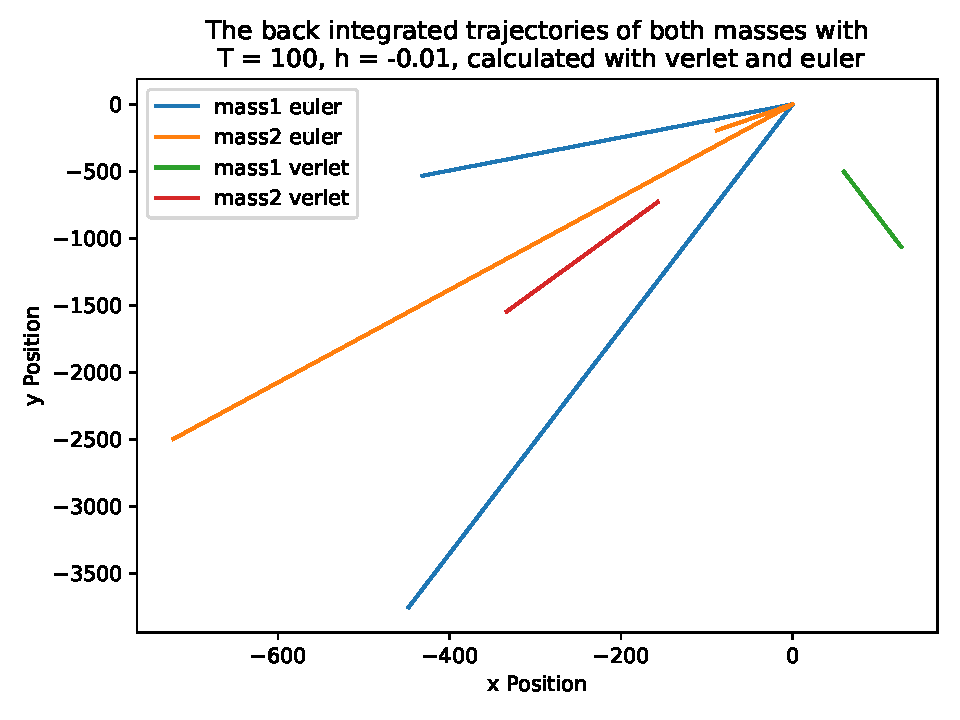
\includegraphics[width=\textwidth]{plots/plotsT_100_h_001/plotd.pdf}
        \caption{The calculated trajectories with a stepsize of $h=-0.01$ up to the time $T=100$.
        The trajectories of euler and verlet are displayed for bothe masses.
        This figures show just the back integrated trajectories from $T=(-100 - 0)$.}
        \label{}
    \end{figure}
    \begin{figure}
        \centering
        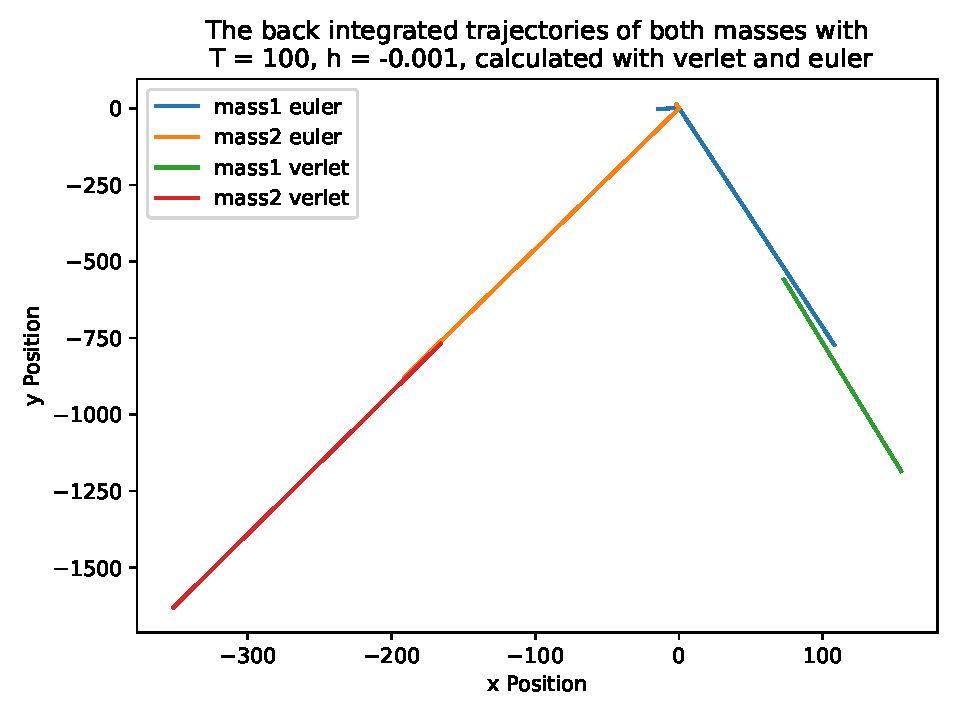
\includegraphics[width=\textwidth]{plots/plotsT_100_h_0001/plotd.pdf}
        \caption{The calculated trajectories with a stepsize of $h=-0.001$ up to the time $T=100$.
        The trajectories of euler and verlet are displayed for bothe masses.
        This figures show just the back integrated trajectories from $T=(-100 - 0)$.}
        \label{}
    \end{figure}
    \begin{figure}
        \centering
        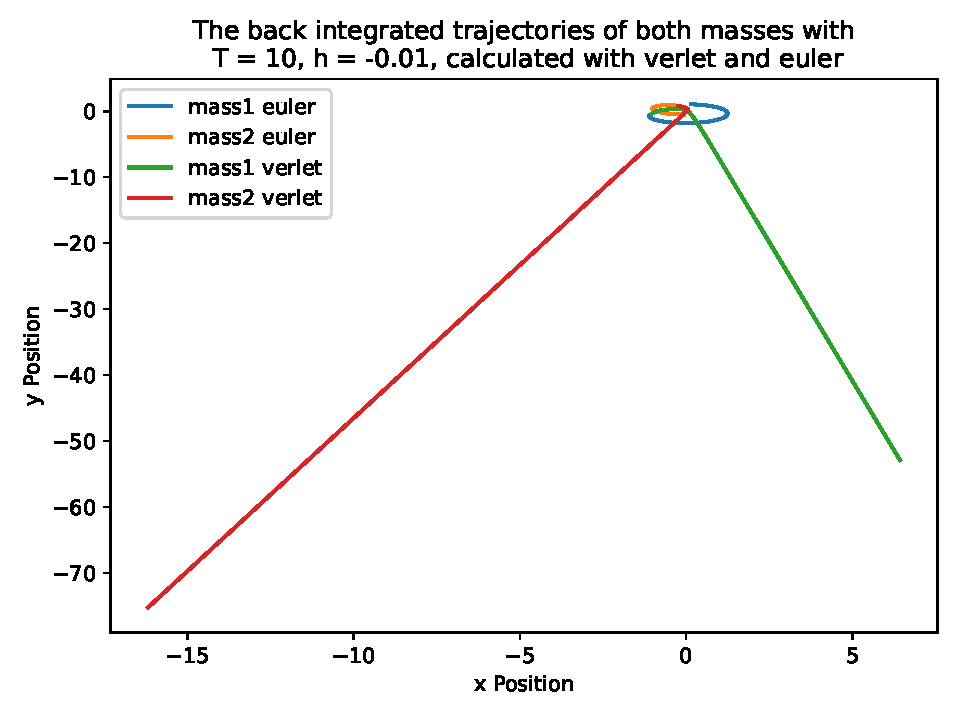
\includegraphics[width=\textwidth]{plots/plotsT_10_h_001/plotd.pdf}
        \caption{The calculated trajectories with a stepsize of $h=-0.01$ up to the time $T=10$.
        The trajectories of euler and verlet are displayed for bothe masses.
        This figures show just the back integrated trajectories from $T=(-100 - 0)$.}
        \label{}
    \end{figure}


\end{itemize}





